\documentclass{beamer}

\usepackage{multirow}

\AtBeginSection[]
{
  \begin{frame}
    \frametitle{Table of Contents}
    \tableofcontents[currentsection]
  \end{frame}
}

\title{Modeling Zombies and Infection}
\author{Ricky Marske and Steven Rosendahl}
\date{}

\usetheme{metropolis}

\begin{document}

\frame{\titlepage}

\section{A Simple Model}

\begin{frame}{Population Decay}
\begin{itemize}
\item Population decay can be modeled by
\[y=a(1-r)^{x}\]
\pause
\item $a:$ Initial amount of population
\pause
\item $r:$ Decay rate
\pause
\item $x:$ The amount of time that has passed
\end{itemize}
\end{frame}

\begin{frame}{A Zombie Model}
\begin{itemize}
\item Population decay model is a good starting point, but is not strong enough to model zombie
outbreak
\pause
\item Final size population model
\pause
\begin{itemize}
\item Size of the population as $t\to\infty$.
\pause
\item Let $S_{\infty}$ be final size of susceptible population
\pause
\item Let $I_{\infty}$ be final size of infected population
\pause
\item Let $R_{\infty}$ be final size of removed population
\pause
\item Left with the system
\begin{gather*}
\begin{cases}
S'=-\beta(t)SI\\
I'=\beta(t)SI-vI\\
R'=vI
\end{cases}
\end{gather*}
\end{itemize}
\end{itemize}
\end{frame}

\section{Adding Complexity}

\begin{frame}{Probability}
\begin{itemize}
\item In the initial model, we assumed
\pause
\begin{enumerate}
\item Non-Infected would have no response to infected
\pause
\item No one was immune
\pause
\item No one could survive the virus or be cured
\end{enumerate}
\pause We will look at each one of these additional features individually
\end{itemize}
\end{frame}

\begin{frame}{Reaction to Zombies}
\begin{itemize}
\item The heat equation can be used to model the spread of zombies
\pause
\item Happens when humans randomly flee from zombies
\end{itemize}
\[
\frac{\partial Z}{\partial t} (x,t) =
D \frac{\partial^2 Z}{\partial x^2} (x,t) \;\;\;\;\;\; \text{(the partial differential equation)}
\]
\pause
\[
Z(x,0) = \begin{cases}
Z_0 & \text{for $0 \leq x \leq 1$}\\
0 & \text{for $x > 1$}
\end{cases} \;\;\;\;\;\;\ \text{(the initial condition)}
\]
\pause
\[
\frac{\partial Z}{\partial x} (0,t) = 0 =
\frac{\partial Z}{\partial x} (L,t) \;\;\;\;\; \text{(zero-flux boundary condition)}
\]
\noindent\\
\noindent\\
\noindent\\
\pause
\[
Z(x,t) = \frac{Z_0}{L} + \sum_{n=1}^{\infty}
\frac{2Z_0}{n \pi}\sin\left(\frac{n \pi}{L}\right)
\cos\left(\frac{n \pi}{L} x\right) e^{\left(-\left(\frac{n \pi}{L}\right)^2 Dt\right)}
\]
\end{frame}

\begin{frame}{Reaction to Zombies}
\begin{center}

\begin{minipage}{0.4\textwidth}
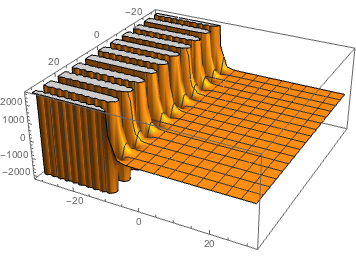
\includegraphics[scale=0.3]{heat_01}\\
$n=1$
\end{minipage}
\begin{minipage}{0.4\textwidth}
\pause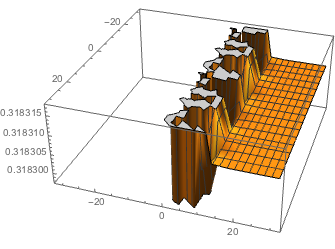
\includegraphics[scale=0.3]{heat_02}\\
$n=100$
\end{minipage}

\begin{minipage}{0.4\textwidth}
\pause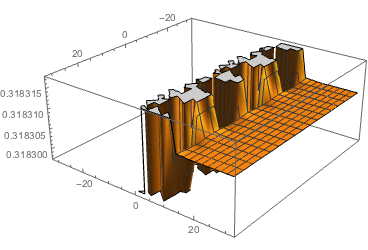
\includegraphics[scale=0.3]{heat_03}\\
$n=500$
\end{minipage}
\begin{minipage}{0.4\textwidth}
\pause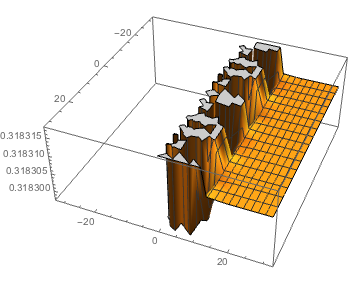
\includegraphics[scale=0.3]{heat_04}\\
$n=1000$
\end{minipage}

\end{center}
\end{frame}

\begin{frame}{Non-Infected Responses}
\begin{itemize}
\item Humans will have a natural response to virus outbreak
\pause
\begin{itemize}
\item One reaction may be to form groups away from the infected
\pause
\item Prevalent in a zombie scenario
\pause
\item Twitch.tv provides a real life example of this
\pause
\item Popular users are like the groups of non-infected
\pause
\item We can analyze what happens when these large groups of non-infected are suddenly hit with the
zombie virus
\end{itemize}
\pause
\item This behavior can be modeled using NetLogo
\end{itemize}
\end{frame}

\begin{frame}{NetLogo Zombie Model}
\begin{itemize}
\item Four different scenarios
\pause
\begin{enumerate}
\item Zombies age and die
\pause
\item Virus dying out in carriers
\pause
\item Vaccination combating virus
\pause
\item Humans dying from old age
\end{enumerate}
\end{itemize}
\begin{center}
\pause
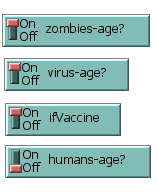
\includegraphics[scale=0.5]{classes}
\hspace{2cm}
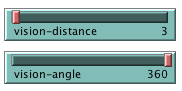
\includegraphics[scale=0.5]{grouping}
\end{center}
\end{frame}

\begin{frame}{Twitch Zombie Outbreak}
\begin{itemize}
\item We created a program to ``infect" twitch users
\pause
\begin{enumerate}
\item Start with initial user/users
\pause
\item Mark all users in that chat as infected
\pause
\item Look through all the infected users
\pause
\begin{itemize}
\item If the user is streaming, then infect all their viewers in their chat
\end{itemize}
\pause
\item Repeat indefinitely
\end{enumerate}
\pause
\item We expect to see bursts of infected after lulls of no infected
\pause
\item This can be modeled by
\[
y=3122.33 + 0.580e^{x}
\]
\end{itemize}
\end{frame}

\begin{frame}{Twitch Zombie Outbreak}
% \hspace{-1cm}
Data From Twitch\hspace{2.5cm}Data From NetLogo
\begin{minipage}{0.5\textwidth}
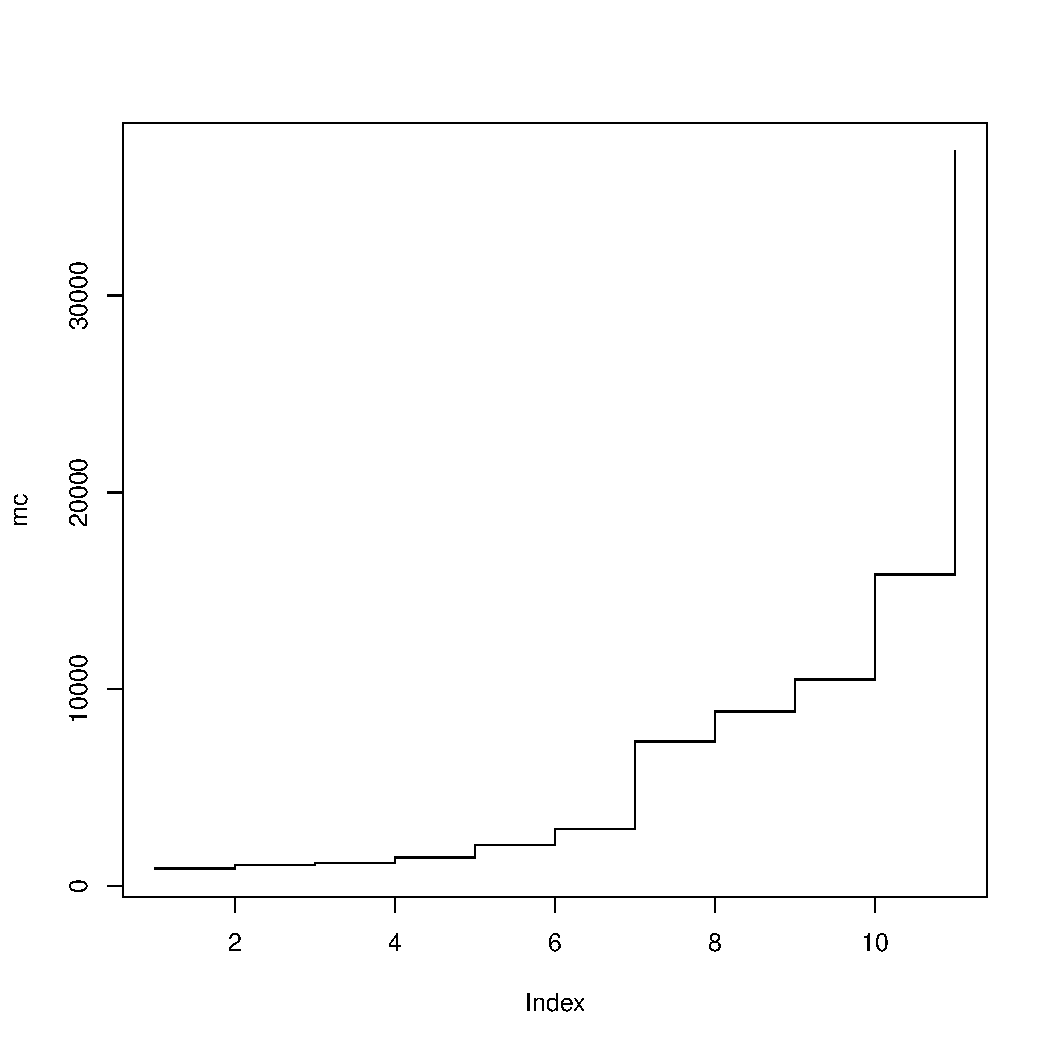
\includegraphics[scale=0.3]{Rplots}
\end{minipage}
\begin{minipage}{0.4\textwidth}
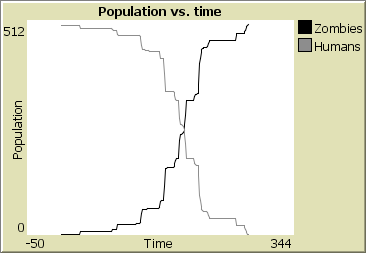
\includegraphics[scale=0.6]{zombie_exponential}
\end{minipage}
\end{frame}

% \begin{frame}{Immunities}
% \begin{itemize}
% % \item Not every person is necessarily susceptible to a disease
% % \pause
% % \item There is a chance that someone in contact with an infected will not become infected
% % \pause
% \item We can model this with a modified version of the Twitch program
% \pause
% \begin{enumerate}
% \item Follow the same procedure again, but mark a user as either infected or immune
% \pause
% \item If the user is immune then they can not infect their users
% \pause
% \item Does not account for carriers of the disease
% \end{enumerate}
% \end{itemize}
% \end{frame}

\begin{frame}{Cures and Survival}
\begin{itemize}
\item The time at which a cure is introduced affects the model
\pause
\item Can be represented by a wave equation:
\[
u_{tt}-k^{2}u_{xx}=0
\]
\pause
\item To show the offset, we have
\[
u_{tt}-k^{2}u_{xx}=\zeta
\]
\pause
\item $\zeta$ represents the time offset
\pause
\item This yields the solution
\[
u(x,t)=\zeta+\sum_{n=1}^{\infty}(k_{1}\sin{t}+k_{2}\cos{t})\sin{n\pi x}
\]
\end{itemize}
\end{frame}

\begin{frame}{Cures and Survival}
\begin{center}

\begin{minipage}{0.4\textwidth}
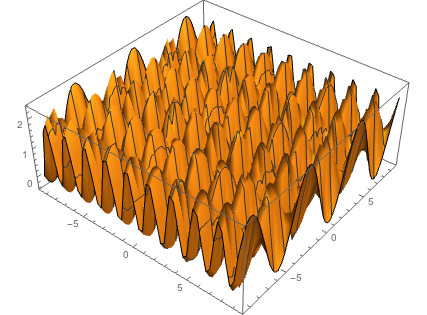
\includegraphics[scale=0.3]{cure_01}\\
$n=1$
\end{minipage}
\begin{minipage}{0.4\textwidth}
\pause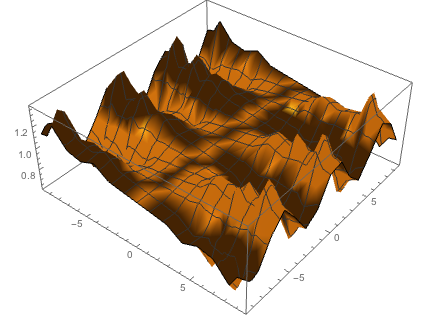
\includegraphics[scale=0.3]{cure_02}\\
$n=100$
\end{minipage}

\begin{minipage}{0.4\textwidth}
\pause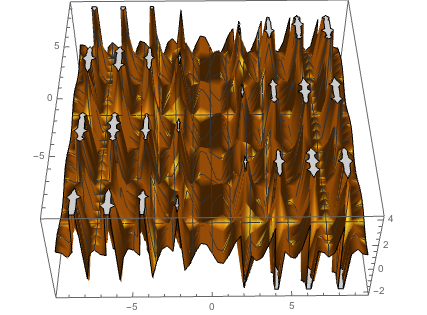
\includegraphics[scale=0.3]{cure_0201}\\
$n=500$
\end{minipage}
\begin{minipage}{0.4\textwidth}
\pause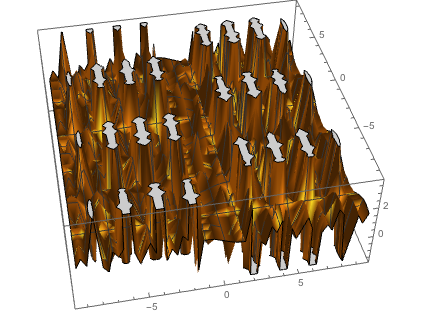
\includegraphics[scale=0.3]{cure_03}\\
$n=1000$
\end{minipage}

\end{center}
\end{frame}

\begin{frame}{Cures and Survival}
\[
u(x,t)=\zeta+\sum_{n=1}^{\infty}(k_{1}\sin{t}+k_{2}\cos{t})\sin{n\pi x}
\]
\begin{itemize}
\item There is a saddle regardless of $\zeta$
\pause
\item The system will move towards the saddle no matter what
\end{itemize}
\end{frame}

\begin{frame}{References}

\end{frame}

\end{document}
